\documentclass[a4paper]{article}
\usepackage{amsthm}
\newtheorem{definition}{Definition}[subsection]
\usepackage[english]{babel}
\usepackage[utf8]{inputenc}
\usepackage{amsmath}
\usepackage{amsfonts}
\usepackage{natbib}
\usepackage{graphicx}
\usepackage{rotating}
\usepackage[colorinlistoftodos]{todonotes}
\usepackage[margin=1in]{geometry}
\renewcommand{\baselinestretch}{2.0}
\setlength{\parindent}{0in} 

\title{OPERATIONAL RISK CONCEPT PAPER}

\author{Mphekeleli Hoohlo}

\date{\today}

\begin{document}
\maketitle

%\begin{abstract}

%This paper applies  in operational risk management (ORM).  %(\texttt{OpRisk}) literature are, given how its importance has increased significantly over the last decades. The gap in the work is addressed %through applications of machine learning techniques on the observed data, which demonstrates how these issues in \texttt{OpRisk} measurement %can be resolved due to their flexibility in obtaining empirical results from primary data.

%\end{abstract}

\section{Introduction}
\label{sec:Introduction}
\subsection{Introduction}

The initial aim of this study is to apply a generalised linear model (GLM) that is suitable for exposure-based operational risk (EBOR) treatments within the operational risk management framework (ORMF), which effectively replaces historical loss severity curves obtained from historical loss counts, by forward-looking measures using event frequencies based on actual operational risk (OpRisk) exposures. Preliminary work on EBOR models was undertaken by \citep{einemann2018operational}. Secondly, the study provides comprehensive computational comparisons of various data-intensive techniques, versus classical statistical estimation methods for classification and regression performances between the two. \medskip

Our understanding of existing ORMF to date is limited to the assumption that financial institutions (FI's) are risk-neutral. In lieu of the afore-mentioned, this study finally seeks to invalidate the risk-neutral assumption, by means of various unsupervised learning techniques, by proposing that FI's are more risk-averse; this can be measured by analysing subtle patterns between data features and trends in the allocated risk capital estimates. In theory, a risk manager who experiences persistent/excessive losses due to particular risk events, would over-compensate cover for these particular risk types, and this would show in reduced losses in these types over time. \medskip

\subsection{Loss collection data exercise (LCDE)}

The main challenge in OpRisk modeling is in poor loss data quantities, and low data quality. There are usually very few data points and are often characterised by high frequency low severity (HFLS) and low frequency high severity (LFHS) losses. It is common knowledge that HFLS losses at the lower end of the spectrum tend to be ignored and are therefore less likely to be reported, whereas low frequency high severity losses (LFHS) are well guarded, and therefore not very likely to be made public. In this study, a new dataset with unique feature characteristics is developed using the official loss data collection exercise (LDCE), as defined by \cite{basel2011operational} for internal data. The dataset in question is at the level of individual loss events, it is fundamental as part of the study to know when they happened, and be able to identify the root causes of losses arising from which OpRisk loss events.\medskip

The LCDE is carried out drawing statistics directly from the trade generation and settlement system, which consists of a tractable set of documented trade detail extracted at the most granular level i.e., on a trade-by-trade basis [as per number of events (frequencies) and associated losses (severities)], and then aggregated daily. The dataset is split into proportions and trained, validated and tested. The afore-mentioned LDCE, is an improved reflection of the risk factors by singling out the value-adding processes associated with individual losses, on a trade-by-trade level.\medskip

\section{An exposure-based OpRisk (EBOR) methodology}

Exposure is residual risk, or the risk that remains after risk treatments have been applied. In the ORMF context, it is defined as:
\begin{definition}
The risk exposure of risk type $i$, $d_i$ is the time interval from the initial moment when the event happened, until the occurrence of a risk correction.  
\end{definition}
By nature it is an OpRisk event type for which there usually is a significant lag between the moment the event is conceived to the moment the event is observed and accounted for. The fundamental premise of the tricky nature behind ORMF, is to provide an exposure-based treatment of OpRisk losses, which caters to modeling capital estimates for forward-looking aspects of ORM due to the lag in the loss data i.e., the gap between the moment the risk is conceived and realised losses. This timing paradox often results in questionable capital estimates, especially for those near misses, pending and realised losses that need to be captured in the model.\medskip

\cite{einemann2018operational}, in a theoretical paper, constructs a mathematical framework for an EBOR model to quantify OpRisk for a portfolio of pending litigations. Their work unearths an invaluable contribution to the literature, discussing a strategy on how to integrate EBOR and LDA models by building hybrid frameworks which facilitate the migration of OpRisk types from a classical to an exposure-based treatment through a quantitative framework, capturing forward looking aspects of business environment and internal control factors (BEICF's) \citep{einemann2018operational}. 

\subsection{Limitations of the EBOR model}

Their model \citep{einemann2018operational} is particularly well-suited to the specific risk type dealt with in their paper i.e., the portfolio of litigation events, due to better usage of existing information and more plausible model behavior over the litigation life cycle, but is bound to under-perform for many other OpRisk event types, since these EBOR models are typically designed to quantify specific aspects of OpRisk -   litigation risk have rather concentrated risk profiles.\medskip

Furthermore, the analytical expression for the loss variable is a complex mathematical expression further contributing to its many \lq\lq moving parts\rq\rq. It depends on ORM strategies whether this is desirable or not. However, EBOR models are important due to wide applicability beyond capital calculation and its potential to evolve into an important tool for auditing process and early detection of potential losses. \quad 

\subsection{Research Objective 1}

To introduce a generalised additive model for location, scale and shape (GAMLSS) framework for OpRisk management, that captures exposures to forward-looking aspects of the OpRisk loss prediction problem, due to deep hierarchies in the features of covariates in the investment banking (IB) business environment, and internal control risk factors (BEICF) thereof.

\section{Modeling OpRisk depending on covariates}

This section of the paper concentrates on combining various supervised learning techniques with extreme value theory (EVT) fitting, which is very much based on the Dynamic EVT-POT model developed by \cite{chavez2016extreme}. This can only happen due to an abundance of larger and better quality datasets and which also benefits the loss distribution approach (LDA) and other areas of OpRisk modeling.  In \cite{chavez2016extreme}, they consider dynamic models based on covariates and in particular concentrate on the influence of internal root causes that prove to be useful from the proposed methodology.    

Motivated by the abundance of data and better data quality, these new data-intensive techniques offer an important tool for ORM and at the same time supporting the call from industry for a new class of EBOR models that capture forward-looking aspects of ORM \citep{embrechts2018modeling}. Three different machine learning techniques viz., decision trees, random forest, and neural networks, will be employed using R. A comprehensive list of user defined variables associated with root causes that contribute to the accumulation of OpRisk events (frequency) has been provided, moreover, a lot can be gained from this dataset as it also bears the impacts of these covariates on the severity of OpRisk. 

\subsection{Loss distribution approach (LDA)}

Twenty-one key risk indicators (kri's) with eight feature groups including person identification, trade origination, root causes and market value sensitivities are in the chosen covariates. For each risk event there is information about: trading risk exposure, trading characteristics, causal factor characteristics and the losses created by these factors. The development, training and validation of the machine learning (ML) models lends itself to this new type of data and requires a higher degree of involvement across operations. Moreover, at this level of granularity the different types of data is particularly suited to exposure-based treatment, and other forward-looking aspects within the OpRisk framework, for improved forecasts of OpRisk losses.\medskip

The aggregated operational losses can be seen as a sum $S$ of a random number $N$ individual operational losses \begin{math} (X_1, \ldots, X_N )\end{math}. The total required capital is the sum of VaR of each BL/ET combination calibrated through the underlying mathematical model whose analytic expression is given by: 

\begin{equation}\label{eqn4}
\mathbf{G}_{\vartheta(t)}(x)=Pr[\vartheta(t)\leq x]=Pr\left(\sum_{n=1}^{N(t)}X_{n} \leq x\right), \qquad \mbox{where} \quad \vartheta(t) = \sum_{n=1}^{N(t)} X_{n}.
\end{equation} 

\begin{math} \mathbf{G}(t)\end{math} can only be obtained numerically using the Monte Carlo method, Panjer's recursive approach, and the inverse of the characteristic function (\cite{frachot2001loss}); \cite{aue2006lda}); \cite{panjer2006operational}; \& others).

\subsection{Research Objective 2}

To test the accuracy of several classes of data-intensive techniques in approximating the weights of the risk factors; i.e., the input features of the model viz., TraderID, UpdatedDay, Desk, etc.  of the underlying value-adding processes, against traditional statistical techniques, in order to separately estimate the frequency and severity distribution of the OpRisk losses from historical data. As a consequence, capital estimates should be able to adapt to changes in the risk profile e.g., upon the addition of new products or varying the business mix of the bank (e.g., terminations, voids,  allocations, etc.) to provide sufficient incentives for ORM to mitigate risk \citep{einemann2018operational}.

\section{Theoretical investigations for the quantification of modern ORM}

Within the variety of relations among risk preferences, people have difficulty in grasping the concept of risk-neutrality. In a market where securities are traded, risk-neutral probabilities are the cornerstone of trade, due to their importance in the law of no arbitrage for securities pricing. Mathematical finance is concerned with pricing of securities, and makes use of this idea: That is, assuming that arbitrage activities do not exist, two positions with the same pay-off must also have an identical market value \citep{gisiger2010risk}. A position (normally a primary security) can be replicated through a construction consisting of a linear combination of long, as well as short positions of traded securities. It is a relative pricing concept which removes risk-free profits due to the no-arbitrage condition.\medskip

This idea seems quite intuitive from an OpRisk management perspective. The fact that one can take internal historical loss data and use this to make a statement on the \texttt{OpRisk} VaR measure for the population, is based on the underlying assumption of risk neutrality. Consider a series of disjoint risky events occurring at times $\tau$ to $\tau + 1$.  We can explore the concept of a two state economy in which value is assigned to gains and losses, rather than to final assets, such that an incremental gain or loss can be realised at state $\tau + 1$, contingent on the probability which positively impacts on the event happening.  \medskip

\subsection{Risk-neutral measure $\mathbb{Q}$}

Risk-neutral probabilities simply enforce a linear consistency for views on equivalent losses/gains, with regard to the shape of the value function. The shape the graph depicts a linear relationship based on responses to gains/losses and value. The risk neutral probability is not the real probability of an event happening, but should be interpreted as (a functional mapping) of the number of loss events (frequency). Suppose we have: $\Theta = \mbox{Gain/Loss}$; $\nu(x) = \mbox{risk event happening}$; and $X = \mbox{Individual gain/loss (or both)}$, then
\begin{eqnarray}\label{eqn3}
\Theta = &\sum_{i=1}^{n}\mbox{Pr}[\nu (x_{i})]*X_i & \\
 \mbox{where} \nonumber\\
&\sum_{i=1}^{n}\mbox{Pr}[\nu (x_{i})] = 1 &\qquad \mbox{and} \qquad \mbox{Pr}[\nu (x_{i})] \geq 0 \quad \forall i\nonumber
\end{eqnarray}         

Note that the random variable $\Theta$ is the sum of the products of frequency and severity for losses (in \texttt{OpRisk} there are no gains).\medskip

This formula is used extensively in actuarial practices, for decisions relating to quantifying different types of risk, in particular in the quantification of value-at-risk (VaR) (a risk measure used to determine capital adequacy requirements, commonly adopted in the banking industry). A quantile of the distribution of the aggregate losses is the level of exposure to risk, expressed as VaR. People exhibit a specific four-fold behaviour pattern when facing risk \citep{shefrin2016behavioral}. There are four combinations of gain/loss and moderate/extreme probabilities, with two choices of risk attitude per combination. OpRisk measurement focuses on only those casual factors that create losses with random uncertainty, for the value adding processes of the business unit.

\subsection{Cluster analysis}

Cluster analysis (CA) is an unsupervised machine learning technique, which sets out to group combinations of covariates according to levels of similarity into clusters. The CA algorithm attempts to optimise homogeneity within data groups, and heterogeneity between groups of observations. Thus, in the context of ORM, CA regroups these combinations of covariates into clusters (so that features within each group are similar to one another, and different from features in other groups), ordering and prioritising the root causes of losses.\medskip

A new and challenging argument can be demonstrated through clustering correlated data objects in the OpRisk dataset, by asserting that clustering should show more than one distinct group. In addition, the more groups of distinct clusters, losses are expected to drop, and losses in distinct clusters should also show a decreasing trend over time, with intensifying exposure. Ultimately, subtle patterns of frequencies and associated severities of losses in the OpRisk data can be revealed.\medskip  

The OpRisk dataset is subdivided for training patterns, validated and tested with the \emph{k}-means clustering algorithm. To achieve this the \emph{k}-means algorithm randomly subdivides the data in k groups. Firstly, each groups mean is found by clustering the centers in the input variable-space of the training patterns. In each cluster within each group, the significant variables' coefficients which determine cluster have set centers closest to the cluster centers generated by the \emph{k}-means clustering algorithm applied to the input vectors of the training data \citep{flake1998square}. These clusters  have centers closest:- as defined by a differential metric i.e., the Euclidean distance, to a relationship (e.g. a linear combination of coefficients and variables) which most accurately predicts the target variable.

\subsection{Research Objective 3}

To identify potential flaws in the loss distribution approach (LDA) model of ORM by employing CA. The \textit{classical}  LDA model, through a mathematical framework derives a negative pay-off function (loss) based on a risk-neutral measure $\mathbb{Q}$. The study addresses weaknesses in the current LDA model framework, by assuming managerial risk-taking attitudes are more risk averse. More precisely, the goal is to use CA to learn deep hierarchies of features\footnote{A typical approach taken in the literature is to use an unsupervised learning algorithm to train a model of the unlabeled data and then use the results to extract interesting features from the data \citep{coates2012learning}} found during operations, to then determine whether risk adverse techniques over-compensate for persistent loss event types over time. \medskip

\section{Results: research question 1}

\subsection{Description of the dataset}

The data set contains 2330 3-month risk correction detail, in the interval 01 January - 31 March 2013. For each transaction, there is information about: trading risk exposure, trading characteristics, causal factor characteristics and the losses created by these factors. The exposure variable shows the length of the time interval from the initial moment when the risk event happened, until the occurrence of a risk correction.\medskip

The characteristics of the traded transactions or of the associated risk correction event are given by the following variables: Trade, UpdateTime, UpdatedDay, TradedTime, TradedDay, Desk, CapturedBy, TradeStatus, TraderId, Instrument, Reason behind the risk correction event, Nominal, FloatRef floating rate reference for fixed income products, ResetDate and ResetRate, Theta, Loss severity, four EventTypeCategoryLevel viz., EL1 - Internal Fraud, EL4 - Clients, Products and Business Practices, EL6 - Business Disruption and System Failures, and EL7 - Execution, Delivery, and Process Management  \& all seven associated  BusinessLineLevel, and a binary variable called LossIndicator indicating a $1$ if a realised loss occurs and $0$ for those pending, or near misses.

\subsection{Exploratory data analysis}

\begin{figure}
\begin{frame}
      \centering
       \begin{tabular}{cc}
        \textbf{Intra-day Trend of Loss Severity} & \textbf{Trends of Loss Severities per Trader} \\
        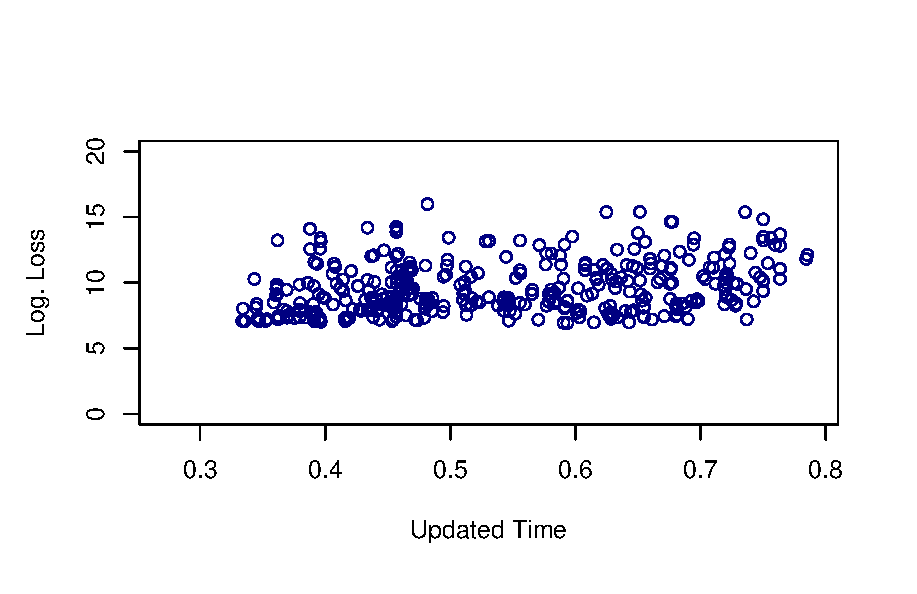
\includegraphics[width=7.5cm]{Rplot.eps}
         &
         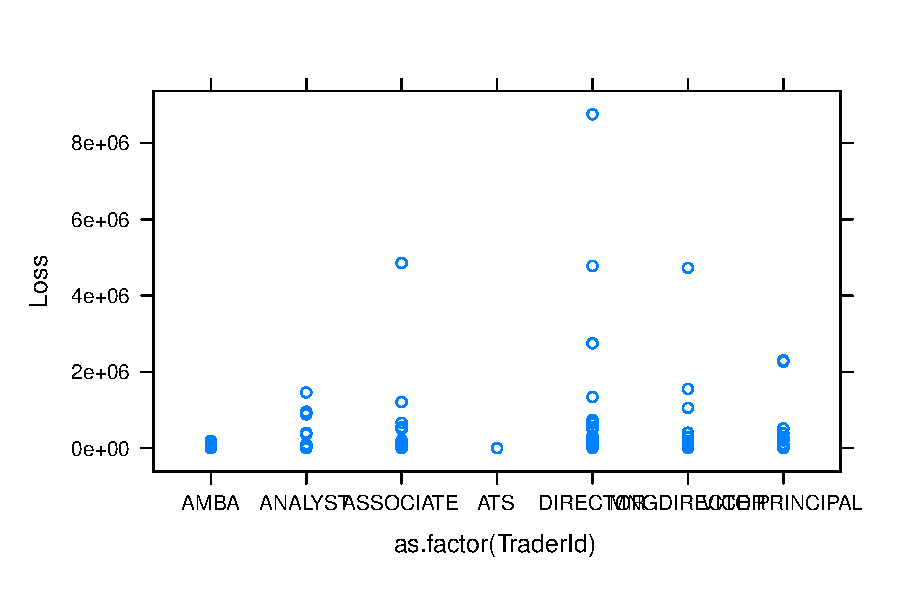
\includegraphics[width=7cm]{Rplot01.eps}
         \end{tabular}
    \end{frame}
    \caption{Intra-day and person identification trends analyses for (Logs of) loss severities}
    \label{Fig1}
\end{figure}

\begin{figure}
\centering

\includegraphics[scale=0.7]{Rplot04.eps}
\caption[Mosaic Plot for Losses]{A mosaic plot for capturing person identification and near miss and/or realised losses}
\label{Fig2}
\end{figure}


\begin{figure}
\begin{frame}
      \centering
       \begin{tabular}{cc}
        \textbf{Histogram of Monthly Loss Frequencies} & \textbf{Histogram of Monthly Trade Frequencies} \\
        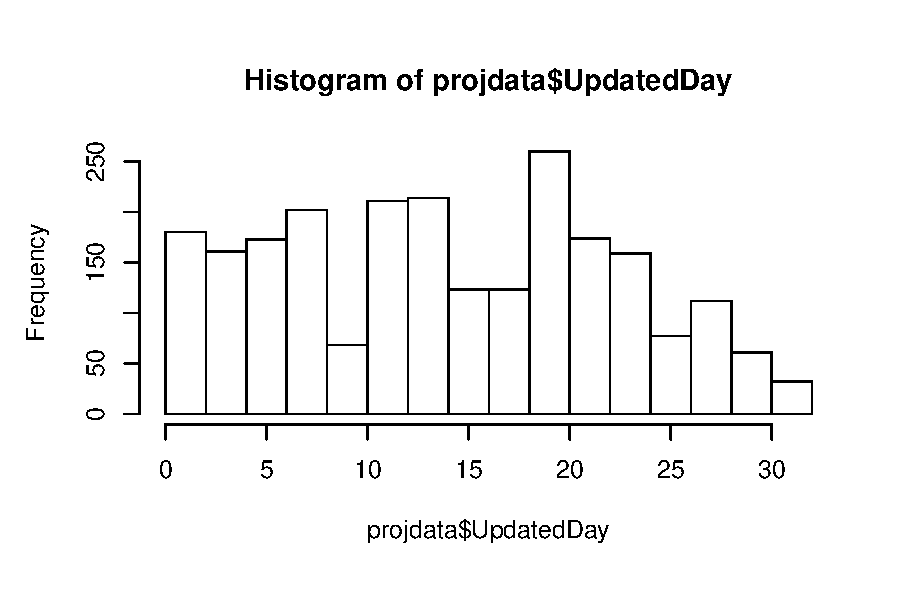
\includegraphics[width=7.5cm]{Rplot02.eps}
         &
         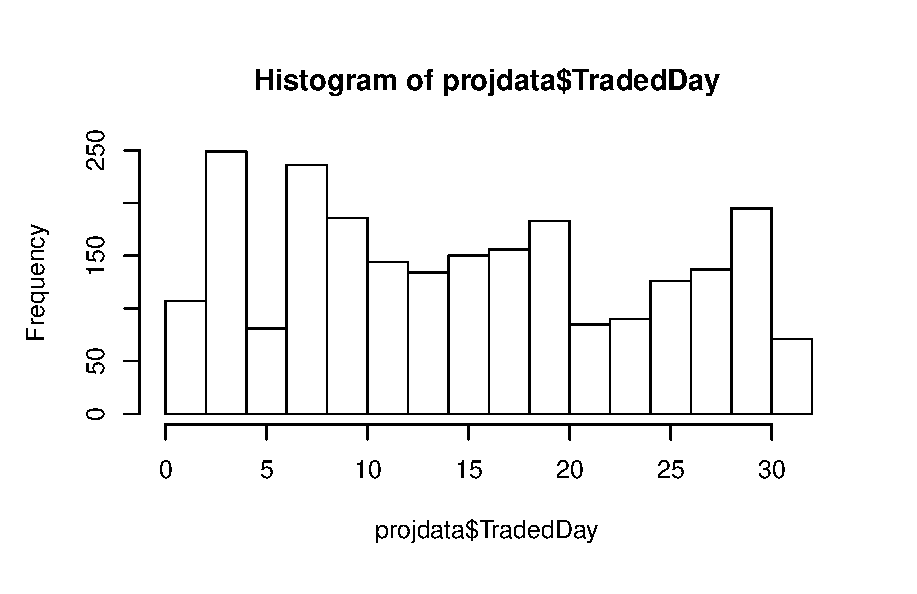
\includegraphics[width=7cm]{Rplot03.eps}
         \end{tabular}
    \end{frame}
    \caption{Histograms showing the totals of the number loss corrections and the number of trades per month}
    \label{Fig3}
\end{figure}
\subsection{The estimation of the Poisson classification models}

The mean daily loss frequency in the risk correction statistics is estimated through Poisson classification models. The target variable is LossIndicator, a binary variable indicating a $1$ if a realised loss occurs and $0$ for those pending or near misses. Suppose that the LossIndicator variable follows a Poisson distribution, so that we aim to estimate the mean frequency through a Poisson classification model using the glm function.  Let us consider a model where the LossIndicator is the target variable:
\begin{verbatim}
fit <- glm(LossIndicator ~ UpdatedDay + UpdatedTime + TradedDay + TradedTime
 + Desk + CapturedBy + TradeStatus + TraderId + Instrument + Reason + Nominal
 + Theta + EventTypeCategoryLevel.1 + BusinessLineLevel1,
 data=d1, family=poisson(link = 'log'), offset = log(exposure))
summary(fit)
\end{verbatim}
The program and output of the estimation is presented below, where many of the covariates are found to be significant predictors.

\subsubsection{R program code}

\begin{verbatim}
options(scipen = 999)
# Load packages
library(rattle, quietly = TRUE)
library(magrittr, quietly = TRUE)
library(Hmisc, quietly = TRUE)
library(chron, quietly = TRUE)
library(dplyr, quietly = TRUE)

# Set parameter values
crv$seed <- 42 # set random seed
crv$taining.proportion <- 0.7 # proportion of data used for training
crv$validation.proportion <- 0.15 # proportion of data used for validation
# Load data
d <- read.csv("OPriskDataSet_exposure.csv",
              sep=";",
              dec=",",
              na.strings=c(".", "NA", "", "?"),
              strip.white=TRUE, encoding="UTF-8")
exposure <- d[,ncol(d)] 
summary(d)
getmode <- function(x){
  u <- unique(x)
  as.integer(u[which.max(tabulate(match(x,u)))])
}
fit <- glm(LossIndicator ~ UpdatedDay + UpdatedTime + TradedDay + TradedTime
 + Desk + CapturedBy + TradeStatus + TraderId + Instrument + Reason + Nominal
 + Theta + EventTypeCategoryLevel.1 + BusinessLineLevel1,
 data=d1, family=poisson(link = 'log'), offset = log(exposure))
summary(fit)  
newdata <- c(UpdatedDay = "23", UpdatedTime = "0,454931", TradedDay = "14",
 TradedTime = "0,194664352", Desk = "Africa", Instrument = "Bill", CapturedBy
  = "PROD CONTROLLER", TraderId = "ATS", TradeStatus = "BO Confirmed", 
Reason = "Fees/Commissions Related", Nominal = "0", Theta = "14,2898465",
 EventTypeCategoryLevel.1 = "EL4", BusinessLineLevel1 = "BL6")

# The Y intercept gives the frequency at which losses occur without any predictors
\end{verbatim}
\subsubsection{Results of the Poisson classification model}
\begin{verbatim}
Call:
glm(formula = LossIndicator ~ UpdatedDay + UpdatedTime + TradedDay + 
    TradedTime + Desk + CapturedBy + TradeStatus + TraderId + 
    Instrument + Reason + Nominal + Theta + EventTypeCategoryLevel.1 + 
    BusinessLineLevel1, family = poisson(link = "log"), data = d1, 
    offset = log(exposure))

Deviance Residuals: 
    Min       1Q   Median       3Q      Max  
-3.9551  -0.4697  -0.1760  -0.0150   3.6624  

Coefficients:
                  Estimate       Std. Error z value        Pr(>|z|)    
(Intercept)                  4.7254503502183  1.6261322314185   2.906        0.003661 ** 
UpdatedDay                   0.0053231234465  0.0093872461817   0.567        0.570674    
UpdatedTime                  0.0639841686234  0.6132264695669   0.104        0.916899    
TradedDay                   -0.0069047563283  0.0071904746324  -0.960        0.336922    
TradedTime                   0.4731206958048  0.4617924382352   1.025        0.305585    
DeskBonds/Repos             -1.0685956222587  0.6008568971048  -1.778        0.075330 .  
DeskCommodities             -2.6309217852537  0.5842787314933  -4.503 0.0000067046966 ***
DeskDerivatives             -1.8795864460055  0.6408185023994  -2.933        0.003356 ** 
DeskEquity                  -2.0348673821173  0.5609592633513  -3.627        0.000286 ***
DeskManagement/Other        -5.1281332087636  1.2582777885752  -4.076 0.0000459121195 ***
DeskMM                      -1.3248568041993  0.5718613219040  -2.317        0.020518 *  
DeskPrime Services          -5.2603436370691  1.2803870696655  -4.108 0.0000398407757 ***
DeskRates                   -3.0151816941130  0.5572104192783  -5.411 0.0000000626009 ***
DeskSND                     -2.9672358183546  0.8145640640906  -3.643        0.000270 ***
CapturedByPROD ACCOUNTANT   -0.4366963208876  0.5998297977370  -0.728        0.466593    
CapturedByPROD CONTROLLER    0.7193042959616  0.4189647801361   1.717        0.086005 .  
CapturedByTECHSUPPORT        0.6484178663160  0.3345056297569   1.938        0.052570 .  
CapturedByUNAUTHORISED       -2.0837491931679  0.6485750481476  -3.213        0.001314 ** 
TradeStatusBO Confirmed      1.0569121175713  0.2141146385318   4.936 0.0000007966049 ***
TradeStatusTerminated        3.9070441221846  1.2491609522646   3.128        0.001762 ** 
TraderIdANALYST             -1.5800866445312  0.5807548279680  -2.721        0.006513 ** 
TraderIdASSOCIATE           -2.0108649332279  0.5932868720315  -3.389        0.000701 ***
TraderIdATS                  0.4338969746887  0.7551902800914   0.575        0.565594    
TraderIdDIRECTOR            -1.4533202194087  0.5839603054409  -2.489        0.012820 *  
TraderIdMNGDIRECTOR         -1.4127430322446  0.5886141359014  -2.400        0.016390 *  
TraderIdVICE PRINCIPAL      -0.6694884247136  0.5883849068645  -1.138        0.255187    
InstrumentBond              -0.0793160744547  0.7456351757064  -0.106        0.915286    
InstrumentBuySellback       -0.8761494395461  0.8428563475231  -1.040        0.298572    
InstrumentCall Deposit      -0.9367652999563  0.6785671781721  -1.381        0.167431    
InstrumentCombination       -1.9633967323079  1.3121037936116  -1.496        0.134556    
InstrumentCreditDefaultSwap -2.0644030499884  0.8189266483920  -2.521        0.011707 *  
InstrumentCurr              -1.1280177017516  0.7609811390681  -1.482        0.138255    
InstrumentCurrSwap          -0.6579224397606  0.7613884434482  -0.864        0.387528    
InstrumentDeposit           -0.0269876513097  0.7049756739758  -0.038        0.969463    
InstrumentEquityIndex       -1.6294697793144  1.2233262225344  -1.332        0.182860    
InstrumentETF                2.8954022524109  1.1308810366054   2.560        0.010458 *  
InstrumentFRA               -3.1382325955602  1.1296442806964  -2.778        0.005468 ** 
InstrumentFRN                0.0571911432211  0.7708593827686   0.074        0.940858    
InstrumentFuture/Forward    -0.5036364308090  0.7341674370884  -0.686        0.492715    
InstrumentIndexLinkedBond   -1.1484618136317  0.8276454277790  -1.388        0.165251    
InstrumentIndexLinkedSwap   -0.8165026000664  0.7597184248051  -1.075        0.282489    
InstrumentOption            -0.2155830392016  0.7768133514213  -0.278        0.781379    
InstrumentOther             -0.5572555430337  0.6868475013595  -0.811        0.417180    
InstrumentRepo/Reverse      -0.5827779068184  0.7979460024797  -0.730        0.465178    
InstrumentSecurityLoan      -1.0841895857261  0.6947091260867  -1.561        0.118609    
InstrumentStock             -2.5885278682373  1.6095678704663  -1.608        0.107789    
InstrumentSwap              -0.4045441939962  0.6895978370286  -0.587        0.557447    
InstrumentTotalReturnSwap   -0.5742577470660  0.7227938948370  -0.794        0.426906    
ReasonBrokerage Related     -3.8071807162651  1.3468950177131  -2.827        0.004704 ** 
ReasonCalendar Related      -1.7692067631568  1.0827638987206  -1.634        0.102265    
ReasonCapture Errors        -2.5887075409606  1.1068756705057  -2.339        0.019348 *  
ReasonClient Request        -4.0283779399856  1.3084582122103  -3.079        0.002079 ** 
ReasonCommodities Delivery   1.1731313722443  1.3275000496677   0.884        0.376850    
ReasonCorrected Reset Level -6.3223973532848  1.0173261089513  -6.215 0.0000000005142 ***
ReasonCPI Fixings           -6.6160591366760  1.0229180416150  -6.468 0.0000000000994 ***
ReasonEarly Termination     -6.1483760049717  0.9342764279199  -6.581 0.0000000000468 ***
ReasonFees/Commissions      -4.6899676586516  1.2692274330654  -3.695        0.000220 ***
ReasonOperations request    -4.3365415267171  1.0927968663212  -3.968 0.0000723883607 ***
ReasonPayments Related      -4.1974133378789  1.1510815566550  -3.646        0.000266 ***
ReasonPortfolio Move        -5.3877964682676  1.3519860066415  -3.985 0.0000674523367 ***
ReasonSales Credits         -0.9417252489155  1.6017509939316  -0.588        0.556576    
ReasonSystem Call Accounts  -7.1905089019106  1.1059143363718  -6.502 0.0000000000793 ***
ReasonTrade enrichment      -2.3463323418684  1.0786724106754  -2.175        0.029615 *  
ReasonTrade Restructure     -8.2221448607904  1.5712008596310  -5.233 0.0000001667516 ***
ReasonTri-Optima            -6.8691140369969  1.6537085111121  -4.154 0.0000327051216 ***
ReasonValuation Group       -2.1004981340857  1.2590298486701  -1.668        0.095247 .  
Nominal                     -0.0000000001983  0.0000000001440  -1.378        0.168326    
Theta                        0.0000001792587  0.0000001010902   1.773        0.076186 .  
EventTypeCategoryLevel.1EL4 -2.1273683247382  0.7722458945102  -2.755        0.005873 ** 
EventTypeCategoryLevel.1EL6  1.6825876304195  0.4254502641732   3.955 0.0000765859573 ***
EventTypeCategoryLevel.1EL7 -3.1914033194679  0.6307379367875  -5.060 0.0000004197121 ***
EventTypeCategoryLevel.1EL8 -6.3580125895837  1.1648933582747  -5.458 0.0000000481470 ***
BusinessLineLevel1BL2       -2.3016556995511  0.6728995111643  -3.421        0.000625 ***
BusinessLineLevel1BL3       -2.0219674382109  0.8698057264209  -2.325        0.020092 *  
BusinessLineLevel1BL4       -3.7787128937891  0.7084552812951  -5.334 0.0000000962128 ***
BusinessLineLevel1BL5       -3.1311086074749  0.7272057735038  -4.306 0.0000166480539 ***
BusinessLineLevel1BL6        1.8762156919229  1.4019719756250   1.338        0.180809    
BusinessLineLevel1BL7        2.5015630317410  1.5700309481337   1.593        0.111088    
BusinessLineLevel1BL9        0.6083370121328  1.7188238248424   0.354        0.723394    
---
Signif. codes:  0 ‘***’ 0.001 ‘**’ 0.01 ‘*’ 0.05 ‘.’ 0.1 ‘ ’ 1

(Dispersion parameter for poisson family taken to be 1)

    Null deviance: 2178.6  on 1181  degrees of freedom
Residual deviance: 1106.0  on 1103  degrees of freedom
  (1148 observations deleted due to missingness)
AIC: 1960

Number of Fisher Scoring iterations: 10
\end{verbatim}

\section{Results: research question 3}

\subsection{Description of the dataset}

The characteristics of the traded transactions or of the associated risk correction event are given by the following variables: Trade, UpdateTime, UpdatedDay, TradedTime, TradedDay, Desk, CapturedBy, TradeStatus, TraderId, Instrument, Reason behind the risk correction event, Nominal, FloatRef floating rate reference for fixed income products, ResetDate and ResetRate, Theta, Loss severity, four EventTypeCategoryLevel viz., EL1 - IF, EL4 - CPBP, EL6 - BDSF, and EL7 - EDPM  \& all seven associated  BusinessLineLevel, and the LossIndicator. The exposure variable shows the length of the time interval from the initial moment when the risk event happened, until the occurrence of a risk correction.\medskip

The data is limited to the training dataset over the interval 01 January - 31 March 2013, in Figure \ref{Fig4}, portrays detail of the trend of OpRisk losses against exposures for each of the 1631 observations and 16 variables. In the first plot, transactions with small exposures are concentrated in the first quadrant where HFLS losses persist. This is in line with the sentiment in risk management circles, that small exposures are not actively managed and hence risk mitigation is not a priority. As a result many of the unforeseeable LFHS losses occur here, as they are not anticipated and therefore slip through OpRisk defences, who more often than not, do not mitigate against these events.\medskip

Loss severities decrease with increasing exposures, as seen by the lowering variabilities (and colour concentration of the exposure) between loses and exposures. This  support the view that more impactful past losses invoke active risk management and mitigation, as risk managers overcompensate for these severities in their management practices i.e., they are more risk averse. In addition there are graphically displayed correlations (which work for numerical explanatory variables only), which are ordered by their strengths. There is a weak positive relationship between exposure and UpdatedDay, TradedTime \& TradedDay; a weak negative relationship with UpdatedTime.  

\subsection{Exploratory data analysis}

\begin{figure}
\begin{frame}
      \centering
       \begin{tabular}{cc}
        \textbf{OpRisk loss severities vs exposure} & \textbf{Ordered correlations by strength} \\
        \includegraphics[width=7cm]{Loss_vs_Exposure(1).eps}
         &
         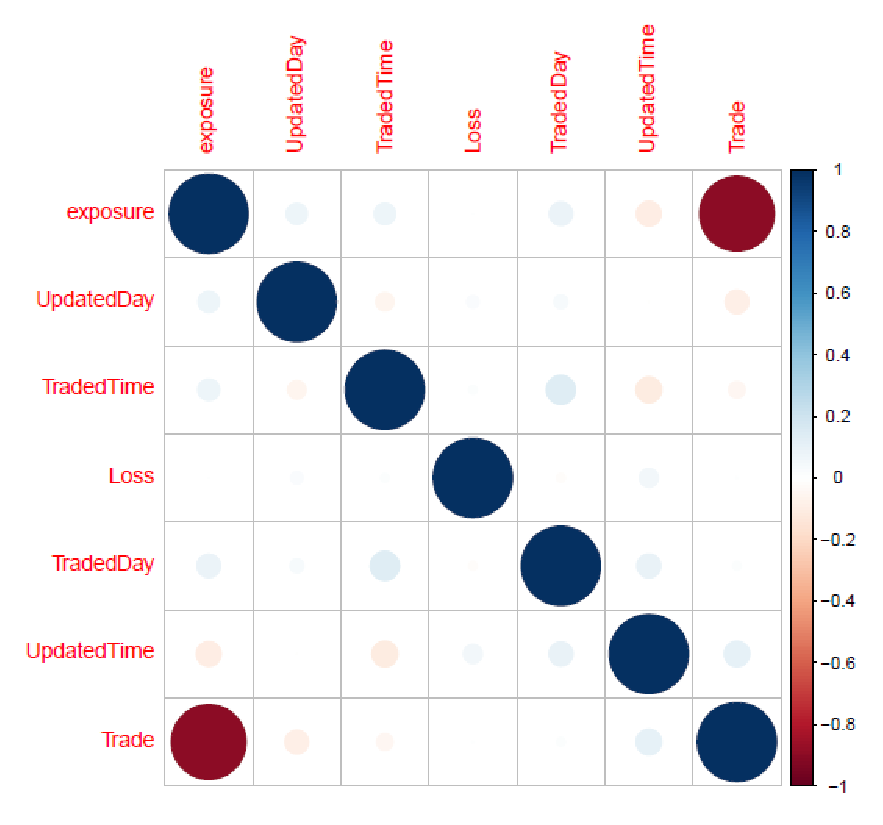
\includegraphics[width=7cm]{CorrPlot.eps}
         \end{tabular}
    \end{frame}
    \caption{Graphically displayed correlations by strength and a plot of OpRisk loss severities vs exposure}
    \label{Fig4}
\end{figure}

\subsection{The estimation of \emph{k}-means clustering algorithm}

A cluster analysis will identify groups within a dataset. The target variable is LossIndicator, a binary variable indicating a $1$ if a realised loss occurs and $0$ for those pending or near misses. The \emph{K}-means clustering algorithm will search for K clusters (specified by the user). The resulting \emph{k} clusters are represented by the mean or average values of each of the variables. Let us consider a model where the LossIndicator is the target variable: The user whose task it is to specify \emph{k}, may guess right or in practice they may obtain a priori, the knowledge of how to select the appropriate \emph{k} in advance.\medskip

Rather than the trial and error method which involves guessing \emph{k} values and successively computing minimum separation between centers, there are several data mining techniques found in the literature, that can be used to determine the optimal \emph{k} \citep{rousseeuw1987silhouettes}. The output plot for the estimation of the optimal \emph{k} is presented in Figure \ref{Fig5} below. We have iterated over cluster sizes from 2 to 10 clusters. The program KMeans resets the random number seed to obtain the same results each time. where the optimal \emph{k} found to be significant close to $\emph{k} = 10$.\medskip

The plot displays the 'sum(withinss)' for each clustering and the change in this value from the previous clustering. The Sum(WithinSS) (blue line) as a performance metric indicates that beyond \emph{k} = 4 clusters the model overfits: Its computes the absolute error which is initially  large, then monotonicaly decreases to the point \emph{k} = 4, it then begins to increase subsequent to the point where the Diffprevious Sum(WithinSS) (red line) intersects viz., at \emph{k} = 4 clusters, which means \emph{k} = 4 is the local optimal number of clusters i.e., beyond which the iterative relative errors converges faster than the absolute errors and successively reduces as \emph{k} increases from 4 to 10.  

\begin{verbatim}
# Rattle timestamp: 2018-12-13 05:23:18 x86_64-w64-mingw32 
# KMeans 
# Reset the random number seed to obtain the same results each time.
set.seed(crv$seed))
\end{verbatim}
\begin{figure}
\centering
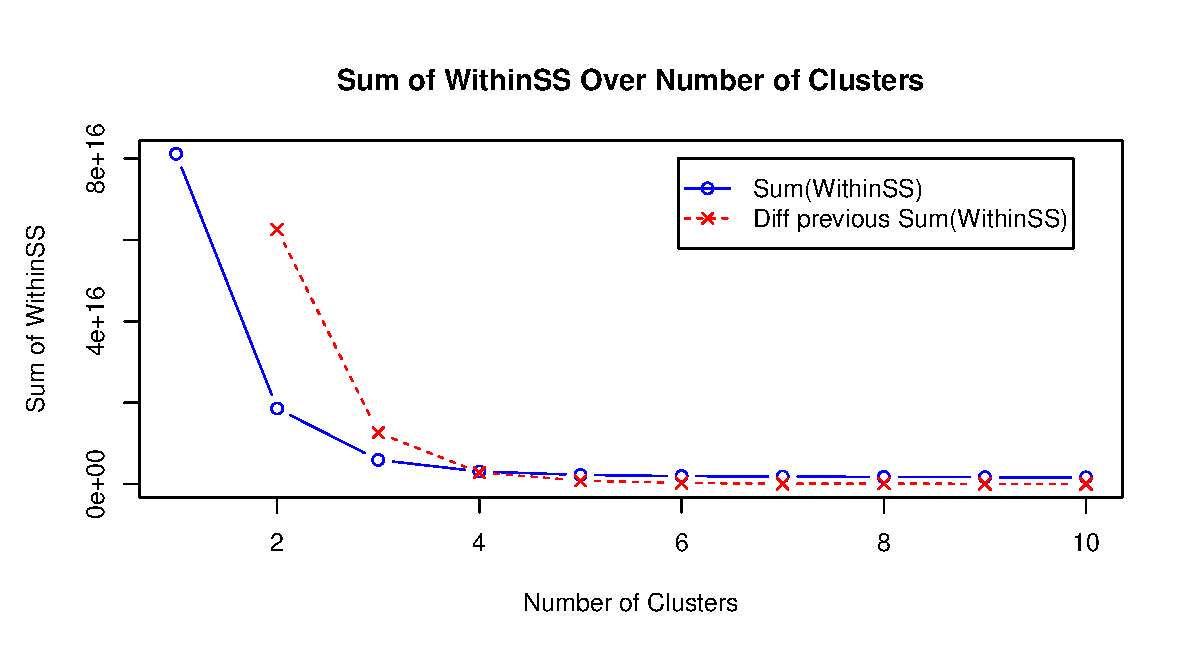
\includegraphics[scale=0.7]{IterateKmeans.eps}
\caption[SS measure]{Finding the optimal number of (\emph{k}) groups by the Silhouette Statistic (SS)}
\label{Fig5}
\end{figure}

\subsubsection{R program code}

\begin{verbatim}
set.seed(crv$seed)
# The 'reshape' package provides the 'rescaler' function.

library(reshape, quietly=TRUE)

# Generate a kmeans cluster of size 4.

crs$kmeans <- kmeans(sapply(na.omit(crs$dataset[crs$sample, crs$numeric]), rescaler, "range"), 4)

#============================================================
# Rattle timestamp: 2018-12-13 07:22:46 x86_64-w64-mingw32 
# Report on the cluster characteristics. 
# Cluster sizes:

paste(crs$kmeans$size, collapse=' ')

# Data means:

colMeans(sapply(na.omit(crs$dataset[crs$sample, crs$numeric]), rescaler, "range"))

# Cluster centers:

crs$kmeans$centers

# Within cluster sum of squares:

crs$kmeans$withinss

# Time taken: 1.86 secs
\end{verbatim}
\subsubsection{Results of the Poisson classification model}
\begin{verbatim}
Cluster sizes:

[1] "478 404 570 179"

Data means:

      Trade  UpdatedDay UpdatedTime   TradedDay  TradedTime 
0.762016409 0.448559166 0.486589314 0.487369712 0.601539912 
       Loss    exposure 
0.003232348 0.121083376 

Cluster centers:

      Trade UpdatedDay UpdatedTime TradedDay TradedTime        Loss
1 0.8106844  0.3943515   0.4123358 0.2912134  0.8556825 0.004692829
2 0.8716248  0.4900990   0.5409218 0.7948845  0.8270263 0.002132631
3 0.8378683  0.4493567   0.5264944 0.4160234  0.2165842 0.002308103
4 0.1431301  0.4970205   0.4351758 0.5443203  0.6397973 0.004757466
    exposure
1 0.08060460
2 0.06359981
3 0.07134609
4 0.51729829

Within cluster sum of squares:

[1]  84.88017  89.27845 148.89661  59.37208

Time taken: 1.86 secs

Rattle timestamp: 2018-12-13 07:22:48 User
\end{verbatim}
\begin{sidewaysfigure}
\centering
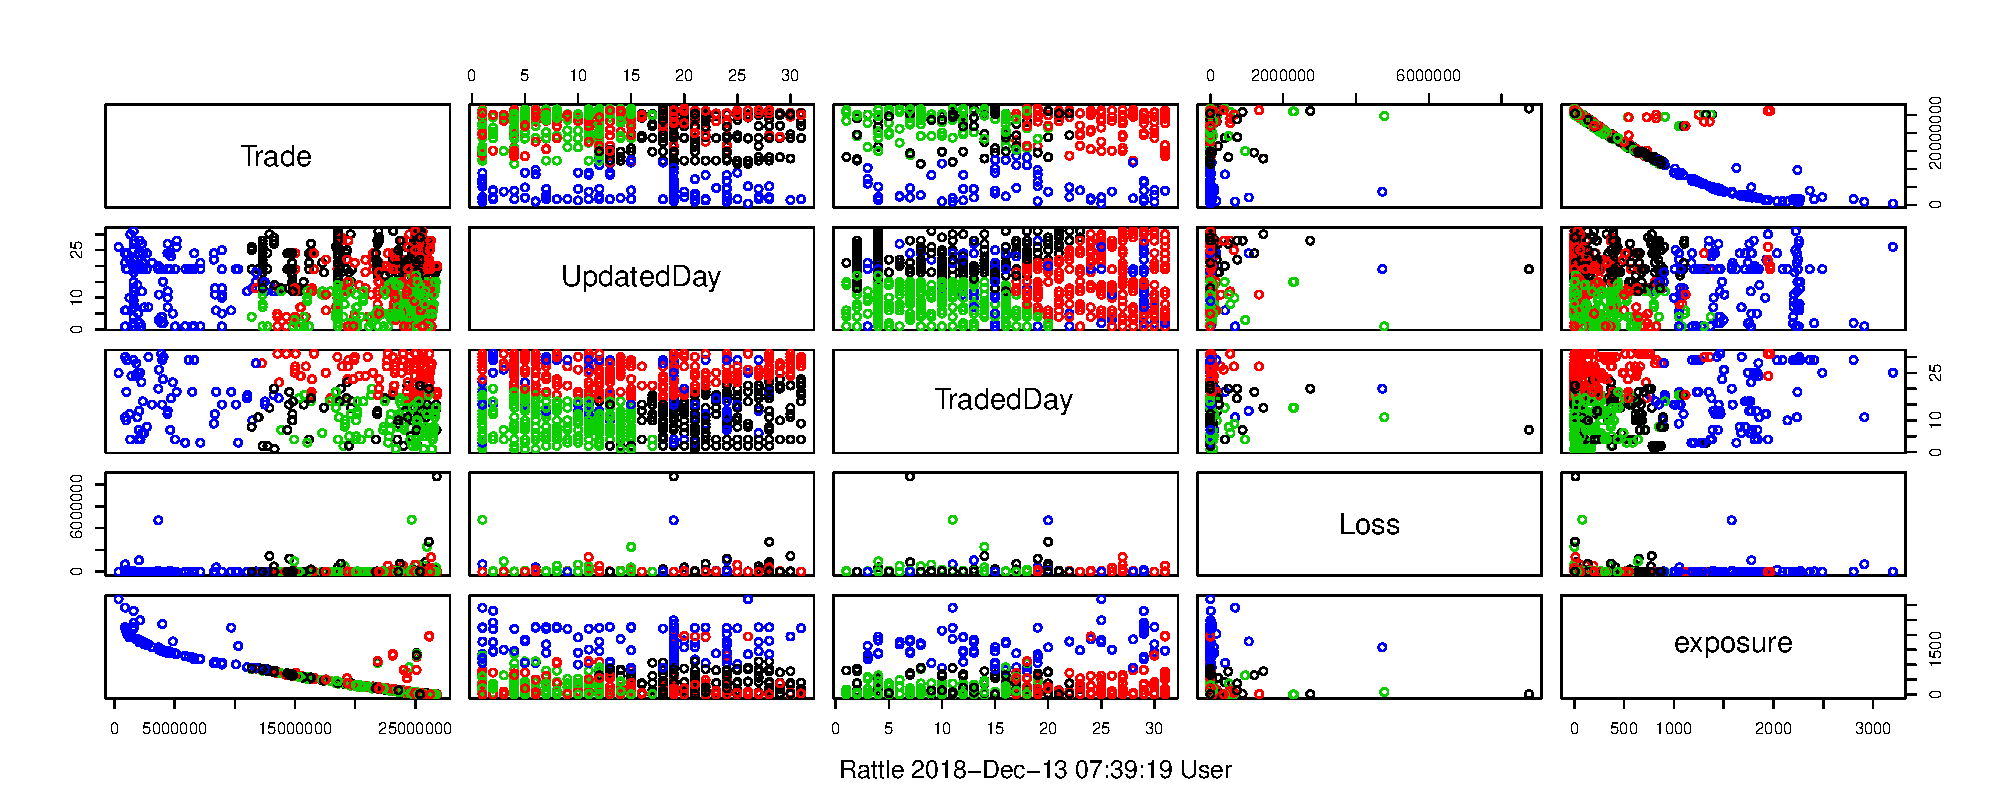
\includegraphics[width=250mm,scale=1.5]{CA14MeansPlot.eps}
\caption[Scatterplot matrix for a \emph{k}-means clustering of size 4]{a scatterplot matrix for the \emph{k}-means clustering of the covariates of frequency loss events consisting of 369 (frequency) loss events amounting to R 61 534 745 (severity) P\&L loss impact.}
\label{Fig6}
\end{sidewaysfigure}
\newpage
\bibliographystyle{apalike}
\bibliography{BiblioGraphy}
\end{document}